    %---------------------------------------------------------------
        %% Jordannetz
        %-----------------------------------------
        \adjustbox{trim=0pt 1.9cm 0pt 0pt,clip}{
        \begin{tikzpicture}[>=stealth', node distance=\layersep cm, shorten >=1pt]
        \def\layersep{1.8}            % vertikal distance between the layers
        \def\neuronsep{1.8}         % Horizontal distance between neurons
        \def\dlsize{2}            % distance between node and layer lable
        \def\inout{\layersep*.65}   % Size of in- and output-arrow
        \def\siz{.8}                % neuronsize
        \def\y{5}                   % Start of the most upper layer
        \def\ni{3}                  % Amount of input neurons
        \def\nh{3}                  % Amount of hidden neurons
        \def\no{2}                  % Amount of output neurons
        \tikzstyle{neuron}=[circle,draw=black,minimum size=\siz cm,inner sep=2pt]
        \tikzstyle{annot} = [text width=6em, text centered]
        \tikzset{fontscale/.style = {font={\fontsize{#1pt}{#1pt}\selectfont}}}
        \newcommand{\neurono}[2][]{
            \node[neuron,circle split,inner sep=2pt] (#1) at (#2)
                    {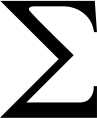
\includegraphics[width=0.225cm]{Bilder/Sigma.png} \nodepart{lower} 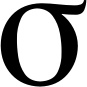
\includegraphics[width=0.225cm]{Bilder/sigma.png}};
        }
        % Draw the input layer nodes
            \foreach \name / \xn in {1,...,\ni}{
                \node[neuron,fontscale=15] (Il-\name) at (\xn*\neuronsep-\neuronsep,\y) {$i_{\xn}$};
                \node[above of=Il-\name, node distance=\inout cm] (Inl-\name) {};
                \draw [->,arrows={-Stealth[length=7pt]},densely dotted] (Inl-\name) edge (Il-\name);
            }
        % Draw the state layer nodes
            \foreach \name / \xn in {2/1,1/2}{
                \node[neuron,fontscale=15] (Sl-\name) at (\xn*\neuronsep-\neuronsep+6,\y) {$s_{\name}$};
            }
        % Draw the hidden layer nodes
            \foreach \name / \xn in {1,...,\nh}{
                \node[neuron] (Hl-\xn) at ({(\ni-1)*\neuronsep/2-\neuronsep/2*(\nh-1)+(\xn-1)*\neuronsep+2.25},\y-\layersep) [fontscale=15] {$h_{\xn}$};
                \node[node distance=\inout cm, below of=Hl-\xn] (Hnl) {};
        % Connect every node in the input/state layer with the hidden layer
                \foreach \source in {1,...,\ni}
                    \draw [->,arrows={-Stealth[length=7pt]}] (Il-\source) edge (Hl-\xn);
             
                \foreach \source in {1,...,2}
                    \draw [->,arrows={-Stealth[length=7pt]}] (Sl-\source) edge (Hl-\xn);    
            }
        % Draw the output layer node
            \foreach \name / \xn in {1,...,\no}{
                \node[neuron] (Ol-\xn) at ({(\ni-1)*\neuronsep/2-\neuronsep/2*(\no-1)+(\xn-1)*\neuronsep+2.25},\y-2*\layersep) [fontscale=15] {$\Omega_{\xn}$};
                ,\y+2*\layersep,
                \node[node distance=\inout cm, below of=Ol-\xn] (Onl) {};
                \draw [->,arrows={-Stealth[length=7pt]},densely dotted] (Ol-\xn) edge (Onl);
        % Connect every node in the hidden/state layer with the output layer
                \foreach \source in {1,...,\nh}
                    \draw [->,arrows={-Stealth[length=7pt]}] (Hl-\source) edge (Ol-\xn);
            }
            \draw[arrows={-Stealth[length=7pt]}, shorten >=1pt, shorten <=1pt] (Ol-2) .. controls (7,1) and  (8,3) .. (Sl-2); 
            \draw[arrows={-Stealth[length=7pt]}, shorten >=1pt, shorten <=1pt] (Ol-1) .. controls (7,-2) and  (10,2) .. (Sl-1);
            \draw[arrows={-Stealth[length=7pt]}, shorten <=1pt] (Sl-1) edge[loop above] ();
            \draw[arrows={-Stealth[length=7pt]}, shorten <=1pt] (Sl-2) edge[loop above] ();
        % Annotate the layers
                \node[annot] (il) at (11,5) {\textbf{Eingabe-/Zustands- schicht}};
                \node[annot,below of=il] (hl) {\textbf{Verdeckte- schicht}};
                \node[annot,below of=hl] {\textbf{Ausgabe- schicht}};
    \end{tikzpicture}
    }